\documentclass[12pt, letterpaper]{article}

\usepackage[utf8]{inputenc}
\usepackage[T1]{fontenc}
\usepackage[spanish]{babel}
\usepackage{geometry}
\usepackage{graphicx}
\usepackage{booktabs}
\usepackage{hyperref}
\usepackage{float}
\usepackage{caption}
\usepackage{subcaption}
\usepackage{enumitem}
\usepackage{parskip}
\usepackage{titlesec}
\usepackage{fancyhdr}
\usepackage{xcolor}
\usepackage{lmodern}
\usepackage{microtype}
\usepackage{csquotes}
\usepackage{tabularx}
\usepackage{array}

\geometry{
  top=2.5cm, bottom=2.5cm,
  left=2.5cm, right=2.5cm
}
\setlength{\headheight}{13.6pt}

\hypersetup{
  colorlinks=true,
  linkcolor=black,
  urlcolor=blue!70!black,
  citecolor=black
}

\pagestyle{fancy}
\fancyhf{}
\fancyhead[L]{\small Visualizaci\'on de Datos -- Semestre I, 2026}
\fancyhead[R]{\small Trabajo Pr\'actico}
\fancyfoot[C]{\thepage}
\renewcommand{\headrulewidth}{0.4pt}

\titleformat{\section}{\large\bfseries}{}{0em}{\thesection.\quad}
\titleformat{\subsection}{\normalsize\bfseries}{}{0em}{\thesubsection.\quad}

\begin{document}

% ── Portada ───────────────────────────────────────────────────────────────────
\begin{titlepage}
  \centering
  \vspace*{1.5cm}

  {\Large\bfseries Universidad T\'ecnica Federico Santa Mar\'ia}\\[0.3cm]
  {\large Departamento de Inform\'atica}\\[0.2cm]
  {\large Visualizaci\'on de Datos -- Semestre I, 2026}

  \vspace{1.5cm}
  \rule{\linewidth}{0.5pt}\\[0.4cm]
  {\LARGE\bfseries Trabajo Pr\'actico: Periodismo de Datos}\\[0.2cm]
  {\large Macrotema: \textit{Muerte} -- Suicidio a nivel mundial}
  \rule{\linewidth}{0.5pt}

  \vspace{1.5cm}

  \begin{tabular}{ll}
    \textbf{Integrante 1:} & Alexis Mellis \\[0.2cm]
    \textbf{Integrante 2:} & Andres Aguila \\
  \end{tabular}

  \vspace{1cm}

  \begin{tabular}{ll}
    \textbf{Profesores:}  & Jos\'e Luis Mart\'i Lara \\[0.2cm]
                          & Wladimir Ormazabal Orellana \\[0.3cm]
    \textbf{Ayudantes:}   & Fernanda Araya Z\'arate \\
                          & Carlos Ar\'evalo Guajardo \\
  \end{tabular}

  \vfill

\end{titlepage}

\tableofcontents
\newpage

% ═════════════════════════════════════════════════════════════════════════════
\section{Introducci\'on y contextualizaci\'on}
% ═════════════════════════════════════════════════════════════════════════════

El presente informe corresponde al Trabajo Pr\'actico del curso de Visualizaci\'on de Datos y constituye la s\'intesis final del macrotema \textbf{Muerte}, con foco en las tasas de suicidio a nivel mundial durante el per\'iodo 1985--2016.

El suicidio es una de las principales causas de muerte prevenible a nivel global. Seg\'un la Organizaci\'on Mundial de la Salud (OMS), m\'as de 700.000 personas mueren por suicidio cada a\~no, lo que lo convierte en la cuarta causa de muerte entre j\'ovenes de 15 a 29 a\~nos a nivel mundial\footnote{World Health Organization. \textit{Suicide worldwide in 2019}. Geneva: WHO; 2021. Disponible en: \url{https://www.who.int/publications/i/item/9789240026643}}. Sin embargo, como se ha evidenciado a lo largo de este trabajo, las percepciones populares sobre el fen\'omeno distan significativamente de la realidad estad\'istica.

A lo largo de tres entregas anteriores se ha construido un hilo conductor que abord\'o el fen\'omeno desde m\'ultiples dimensiones:

\begin{itemize}[nosep]
  \item \textbf{Tarea 1:} An\'alisis exploratorio de la magnitud global del suicidio, su evoluci\'on temporal, distribuci\'on etaria, brecha de g\'enero y concentraci\'on geogr\'afica en los 15 pa\'ises de mayor incidencia. Se evidenci\'o un pico cr\'itico en torno al a\~no 2000, una brecha de g\'enero persistente donde los hombres triplican la tasa femenina, y la paradoja de que los pa\'ises de mayor PIB per c\'apita presentan tasas m\'as elevadas.
  \item \textbf{Tarea 2:} Confrontaci\'on de percepciones populares con la evidencia estad\'istica mediante una encuesta propia. Los resultados revelaron un desconocimiento sistem\'atico: la mayor\'ia cree que los j\'ovenes son el grupo m\'as vulnerable (cuando en realidad son los mayores de 75 a\~nos), que los pa\'ises pobres tienen m\'as suicidios (la relaci\'on es inversa), y que las tasas han aumentado (cuando han disminuido un 7,4\%).
  \item \textbf{Tarea 3:} Visualizaci\'on espacial mediante mapas que confirm\'o la concentraci\'on de las tasas m\'as altas en Europa del Este y Asia Central, y la relaci\'on bivariable entre nivel de ingresos y tasa de suicidios a escala geogr\'afica.
\end{itemize}

Este trabajo final integra las tres etapas previas mediante una selecci\'on de visualizaciones representativas de cada tarea, complementadas con dos nuevas visualizaciones individuales que profundizan en aspectos a\'un no explorados del fen\'omeno.

\subsection{Fuentes de datos}

\begin{itemize}[nosep]
  \item \textbf{Dataset principal:} Kaggle -- \textit{Suicide Rates Overview 1985 to 2016} \\
        Disponible en: \url{https://www.kaggle.com/datasets/russellyates88/suicide-rates-overview-1985-to-2016}
  \item \textbf{Datos de origen:} United Nations Development Programme (UNDP), World Bank, World Health Organization (WHO).
  \item \textbf{Encuesta propia:} Formulario de Google Forms aplicado a 20 personas sobre percepciones del suicidio a nivel mundial (Tarea~2).
  \item \textbf{Referencia contextual:} World Health Organization. \textit{Suicide worldwide in 2019}. Geneva: WHO; 2021.
  % TODO: Agregar fuentes adicionales si se usan nuevos datasets para las visualizaciones nuevas
\end{itemize}

% ═════════════════════════════════════════════════════════════════════════════
\section{Visualizaciones de tareas anteriores}
% ═════════════════════════════════════════════════════════════════════════════

A continuaci\'on se presentan las tres visualizaciones seleccionadas de las entregas previas, una por cada tarea. Estas visualizaciones no ser\'an evaluadas nuevamente, pero se incluye su ficha t\'ecnica como requisito del trabajo pr\'actico.

% ─────────────────────────────────────────────────────────────────────────────
\subsection{Visualizaci\'on 1 -- Tarea 1: Streamgraph de distribuci\'on etaria}
% ─────────────────────────────────────────────────────────────────────────────

\textbf{Autor:} Alexis Mellis \hfill \textbf{Tarea:} Tarea 1

\begin{figure}[H]
  \centering
  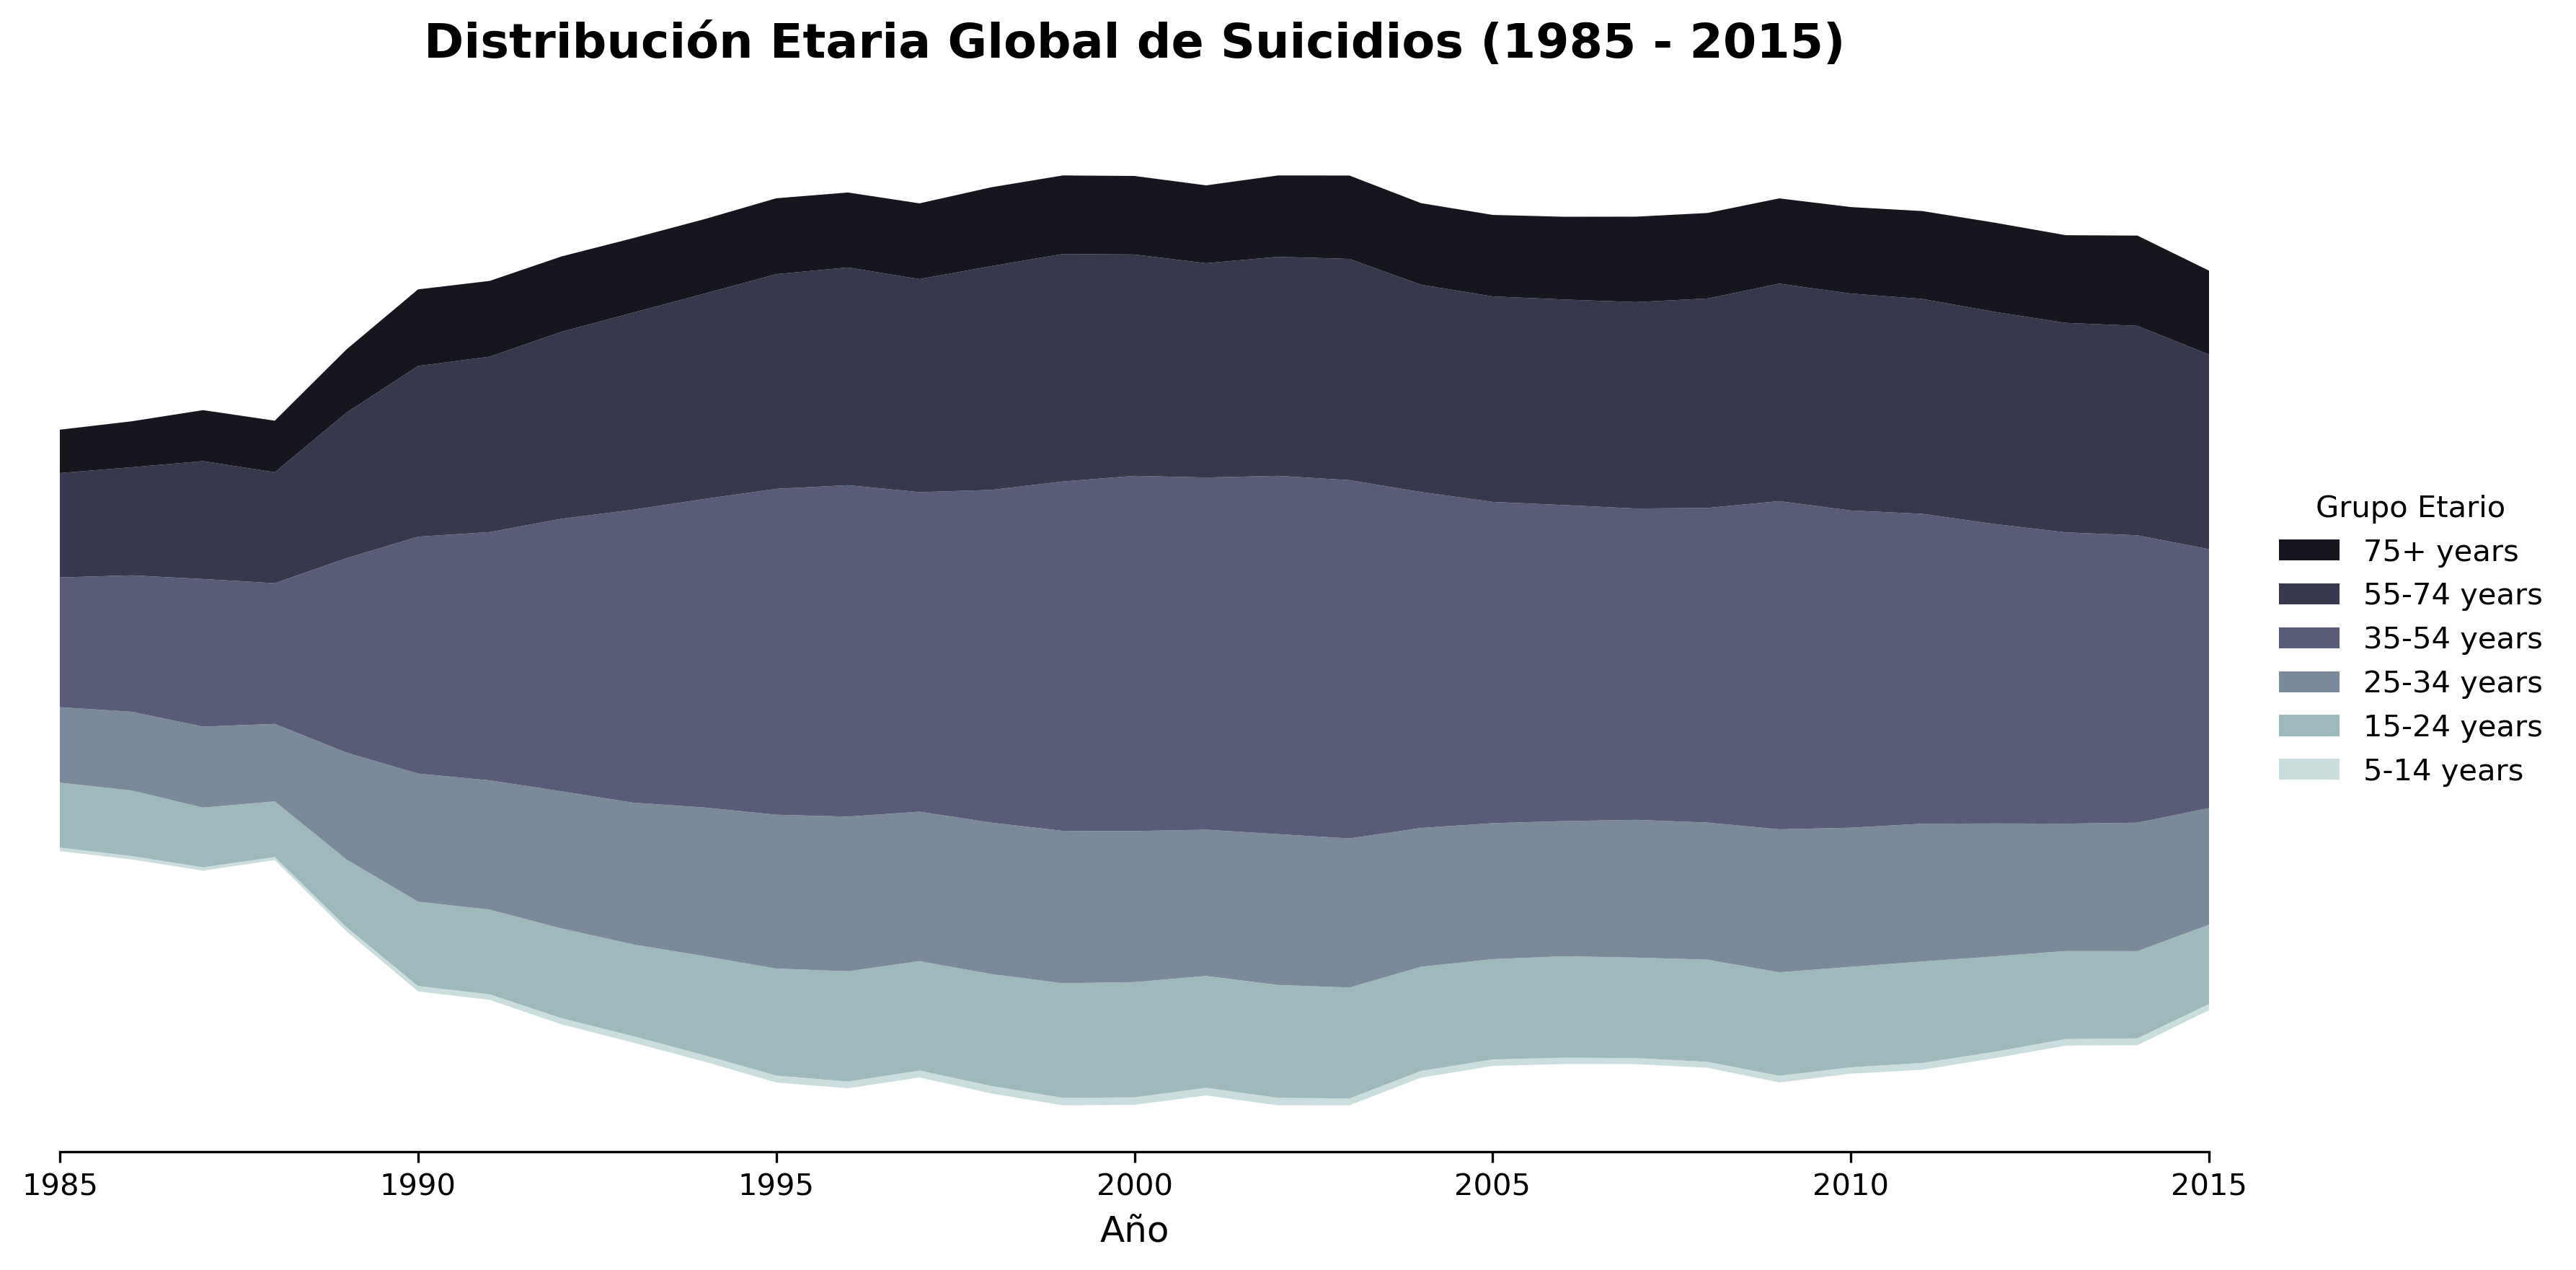
\includegraphics[width=0.85\textwidth]{figures/tarea1_streamgraph.png}
  \caption{Distribuci\'on Etaria Global de Suicidios (1985--2015). Fuente: Kaggle -- Suicide Rates Overview 1985--2016.}
  \label{fig:t1_stream}
\end{figure}

\subsubsection*{Ficha t\'ecnica}

\begin{table}[H]
  \centering
  \begin{tabularx}{\textwidth}{lX}
    \toprule
    \textbf{Elemento} & \textbf{Descripci\'on} \\
    \midrule
    Tipo de gr\'afico & Streamgraph (gr\'afico de flujo apilado) \\
    Marca & \'Area (capas apiladas continuas) \\
    Canal -- Posici\'on X & A\~no (1985--2015), variable temporal ordinal \\
    Canal -- Altura/\'Area & Cantidad total de suicidios por grupo etario, variable cuantitativa \\
    Canal -- Color (matiz) & Grupo etario (6 categor\'ias), variable categ\'orica nominal \\
    Esquem\'atica & Temporal: muestra la evoluci\'on de la composici\'on etaria a lo largo del tiempo \\
    Fuente de datos & Kaggle -- Suicide Rates Overview 1985--2016 \\
    \bottomrule
  \end{tabularx}
\end{table}

% ─────────────────────────────────────────────────────────────────────────────
\subsection{Visualizaci\'on 2 -- Tarea 2: Lollipop Divergente}
% ─────────────────────────────────────────────────────────────────────────────

\textbf{Autor:} Andr\'es \'Aguila \hfill \textbf{Tarea:} Tarea 2

\begin{figure}[H]
  \centering
  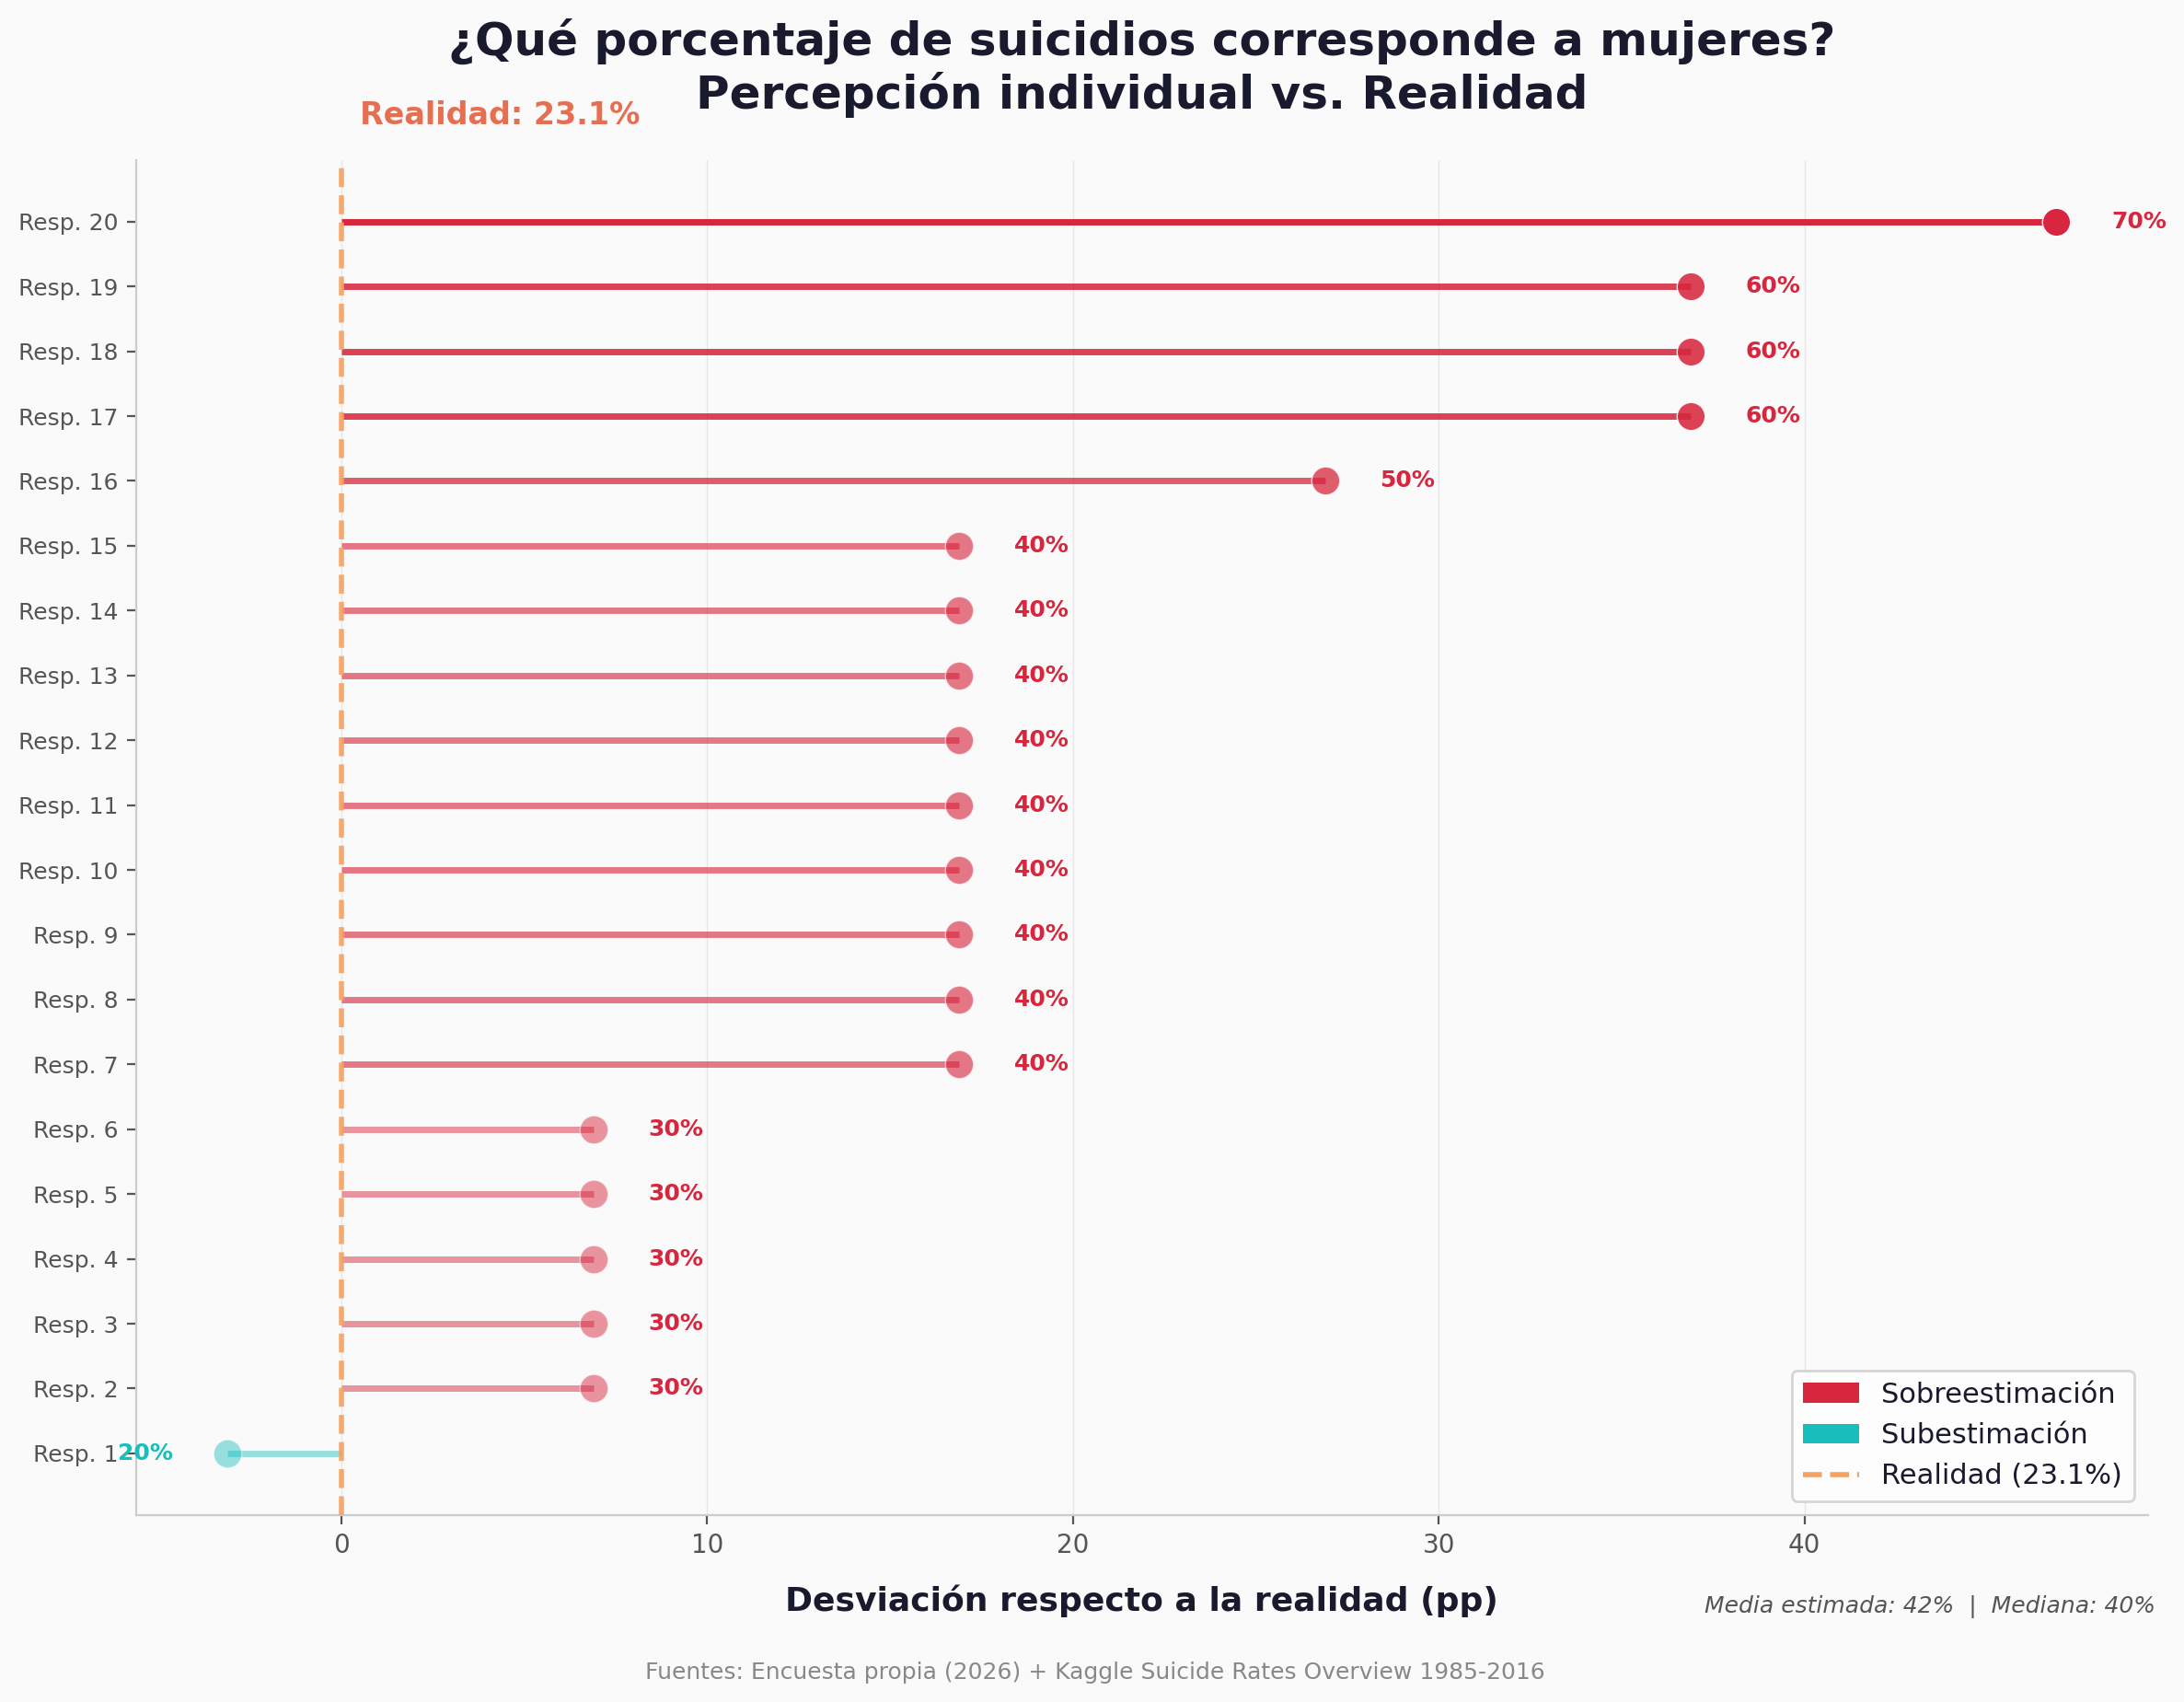
\includegraphics[width=0.85\textwidth]{figures/tarea2_lollipop.png}
  \caption{Lollipop Divergente: Estimaci\'on individual del \% femenino en suicidios vs.\ realidad (23,1\%). Fuentes: Encuesta propia (2026) + Kaggle -- Suicide Rates Overview 1985--2016.}
  \label{fig:t2_lollipop}
\end{figure}

\subsubsection*{Ficha t\'ecnica}

\begin{table}[H]
  \centering
  \begin{tabularx}{\textwidth}{lX}
    \toprule
    \textbf{Elemento} & \textbf{Descripci\'on} \\
    \midrule
    Tipo de gr\'afico & Lollipop Divergente \\
    Marca & Punto (c\'irculo) + L\'inea (tallo) \\
    Canal -- Posici\'on Y & Encuestado individual (categ\'orica nominal) \\
    Canal -- Posici\'on X / Longitud & Desviaci\'on porcentual respecto al valor real (23,1\%), variable cuantitativa \\
    Canal -- Color (matiz) & Direcci\'on de la desviaci\'on: sobreestimaci\'on vs.\ subestimaci\'on, variable categ\'orica binaria \\
    L\'inea de referencia & Valor real del porcentaje femenino en suicidios globales \\
    Esquem\'atica & Comparativa: confronta cada estimaci\'on individual contra el valor real \\
    Fuente de datos & Encuesta propia (2026) + Kaggle -- Suicide Rates Overview 1985--2016 \\
    \bottomrule
  \end{tabularx}
\end{table}

% ─────────────────────────────────────────────────────────────────────────────
\subsection{Visualizaci\'on 3 -- Tarea 3: Mapa Coropleta}
% ─────────────────────────────────────────────────────────────────────────────

\textbf{Autor:} Alexis Mellis \hfill \textbf{Tarea:} Tarea 3

\begin{figure}[H]
  \centering
  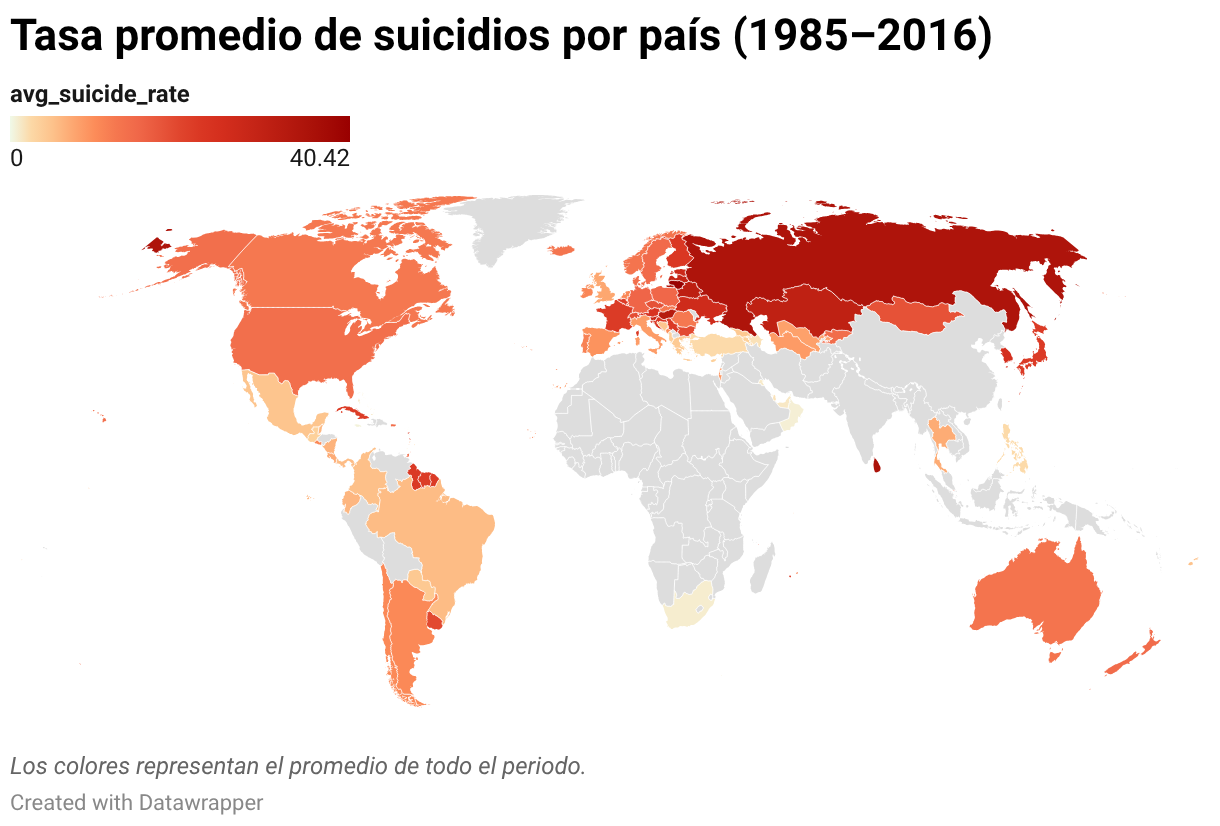
\includegraphics[width=0.95\textwidth]{figures/tarea3_coropleta.png}
  \caption{Mapa coropleta: tasa promedio de suicidios por pa\'is (1985--2016). Fuente: Kaggle -- Suicide Rates Overview 1985--2016.}
  \label{fig:t3_coropleta}
\end{figure}

\subsubsection*{Ficha t\'ecnica}

\begin{table}[H]
  \centering
  \begin{tabularx}{\textwidth}{lX}
    \toprule
    \textbf{Elemento} & \textbf{Descripci\'on} \\
    \midrule
    Tipo de gr\'afico & Mapa Coropleta \\
    Marca & \'Area (pol\'igonos de pa\'ises) \\
    Canal -- Posici\'on & Coordenadas geogr\'aficas (latitud/longitud), variable espacial \\
    Canal -- Color (saturaci\'on) & Tasa promedio de suicidios por 100k hab., escala secuencial de blancos a rojos, variable cuantitativa \\
    Canal -- Color gris & Pa\'ises sin datos disponibles \\
    Esquem\'atica & Descriptiva: muestra la distribuci\'on geogr\'afica de la tasa sin establecer secuencia temporal ni causalidad \\
    Herramienta & Datawrapper \\
    Fuente de datos & Kaggle -- Suicide Rates Overview 1985--2016 \\
    \bottomrule
  \end{tabularx}
\end{table}

% ═════════════════════════════════════════════════════════════════════════════
\section{Nuevas visualizaciones}
% ═════════════════════════════════════════════════════════════════════════════

En esta secci\'on se presentan dos visualizaciones in\'editas que complementan el an\'alisis realizado en las tareas anteriores. Cada integrante desarroll\'o una visualizaci\'on individual.

% ─────────────────────────────────────────────────────────────────────────────
\subsection{Visualizaci\'on 4 -- Nueva: Bump Chart (Alexis Mellis)}
% ─────────────────────────────────────────────────────────────────────────────

\textbf{Autor:} Alexis Mellis \hfill \textbf{Tipo:} Visualizaci\'on individual nueva

\begin{figure}[H]
  \centering
  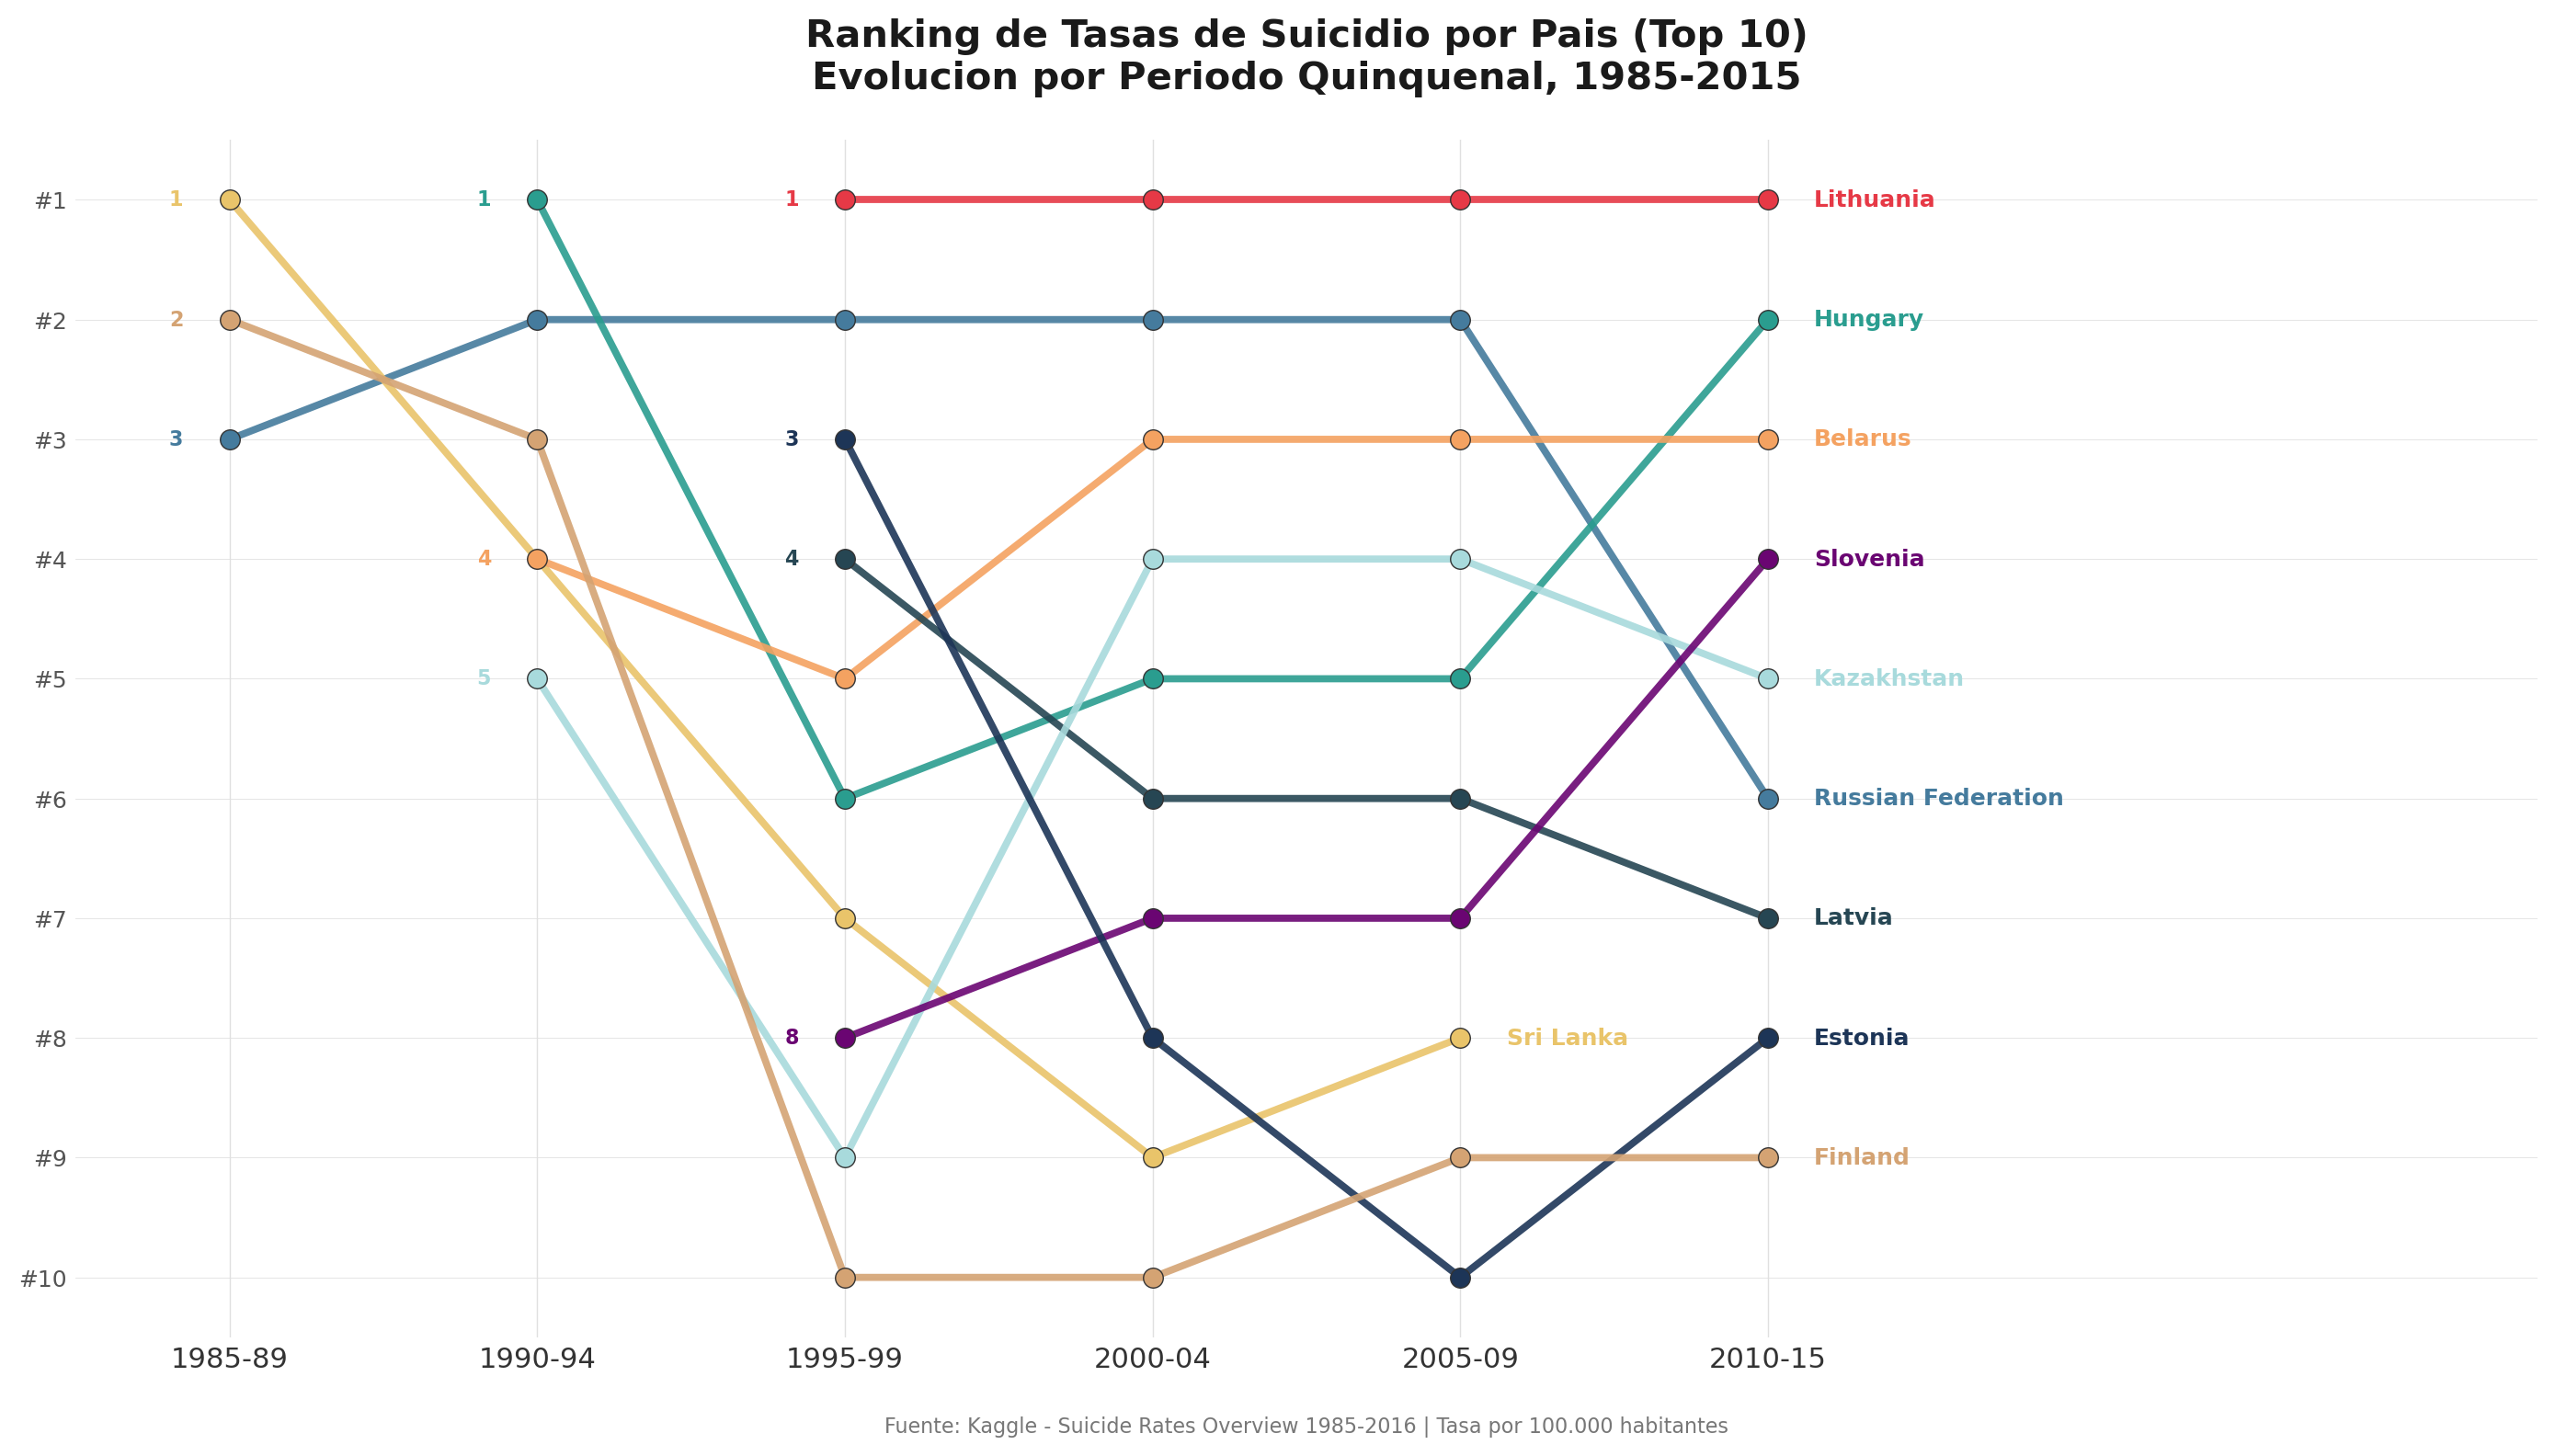
\includegraphics[width=0.95\textwidth]{figures/vis4_bump_chart.png}
  \caption{Bump Chart: Ranking de tasas de suicidio por pa\'is (Top 10), evoluci\'on por per\'iodo quinquenal (1985--2015). Fuente: Kaggle -- Suicide Rates Overview 1985--2016.}
  \label{fig:vis4_bump}
\end{figure}

\subsubsection*{Ficha t\'ecnica}

\begin{table}[H]
  \centering
  \begin{tabularx}{\textwidth}{lX}
    \toprule
    \textbf{Elemento} & \textbf{Descripci\'on} \\
    \midrule
    Tipo de gr\'afico & Bump Chart (gr\'afico de ranking) \\
    Marca & L\'inea (trayectoria de ranking) + Punto (posici\'on por per\'iodo) \\
    Canal -- Posici\'on X & Per\'iodo quinquenal (1985-89 a 2010-15), variable temporal ordinal \\
    Canal -- Posici\'on Y & Posici\'on en el ranking (1 a 10), variable ordinal derivada de la tasa por 100k hab. \\
    Canal -- Color (matiz) & Pa\'is (10 categor\'ias), variable categ\'orica nominal \\
    Esquem\'atica & Temporal-comparativa: muestra c\'omo cambia la posici\'on relativa de los pa\'ises a lo largo del tiempo \\
    Fuente de datos & Kaggle -- Suicide Rates Overview 1985--2016 \\
    \bottomrule
  \end{tabularx}
\end{table}

\subsubsection*{Conclusiones}

\begin{itemize}
  \item Lituania se consolida como el pa\'is con la tasa de suicidio m\'as alta del mundo desde 1995 en adelante, manteniendo el primer puesto del ranking durante cuatro per\'iodos consecutivos. Su ascenso desde la tercera posici\'on en 1985--89 coincide con el colapso de la Uni\'on Sovi\'etica y sus consecuencias socioecon\'omicas.
  \item Se observa un patr\'on claro de ``bloque post-sovi\'etico'': pa\'ises como Lituania, Rusia, Bielorrusia, Letonia, Estonia y Kazajist\'an dominan el Top 10 en todos los per\'iodos, lo que refuerza la hip\'otesis de que la transici\'on geopol\'itica de los a\~nos 90 tuvo un impacto duradero en la salud mental de estas poblaciones.
  \item Hungr\'ia, que lideraba el ranking en 1985--89, presenta una tendencia descendente sostenida, cayendo al segundo puesto en el \'ultimo per\'iodo. Esto sugiere que las pol\'iticas de prevenci\'on implementadas en d\'ecadas recientes han tenido efecto, aunque el pa\'is sigue entre los de mayor incidencia a nivel global.
\end{itemize}

% ─────────────────────────────────────────────────────────────────────────────
\subsection{Visualizaci\'on 5 -- Nueva: Diagrama de Sankey (Andr\'es \'Aguila)}
% ─────────────────────────────────────────────────────────────────────────────

\textbf{Autor:} Andr\'es \'Aguila \hfill \textbf{Tipo:} Visualizaci\'on individual nueva

\begin{figure}[H]
  \centering
  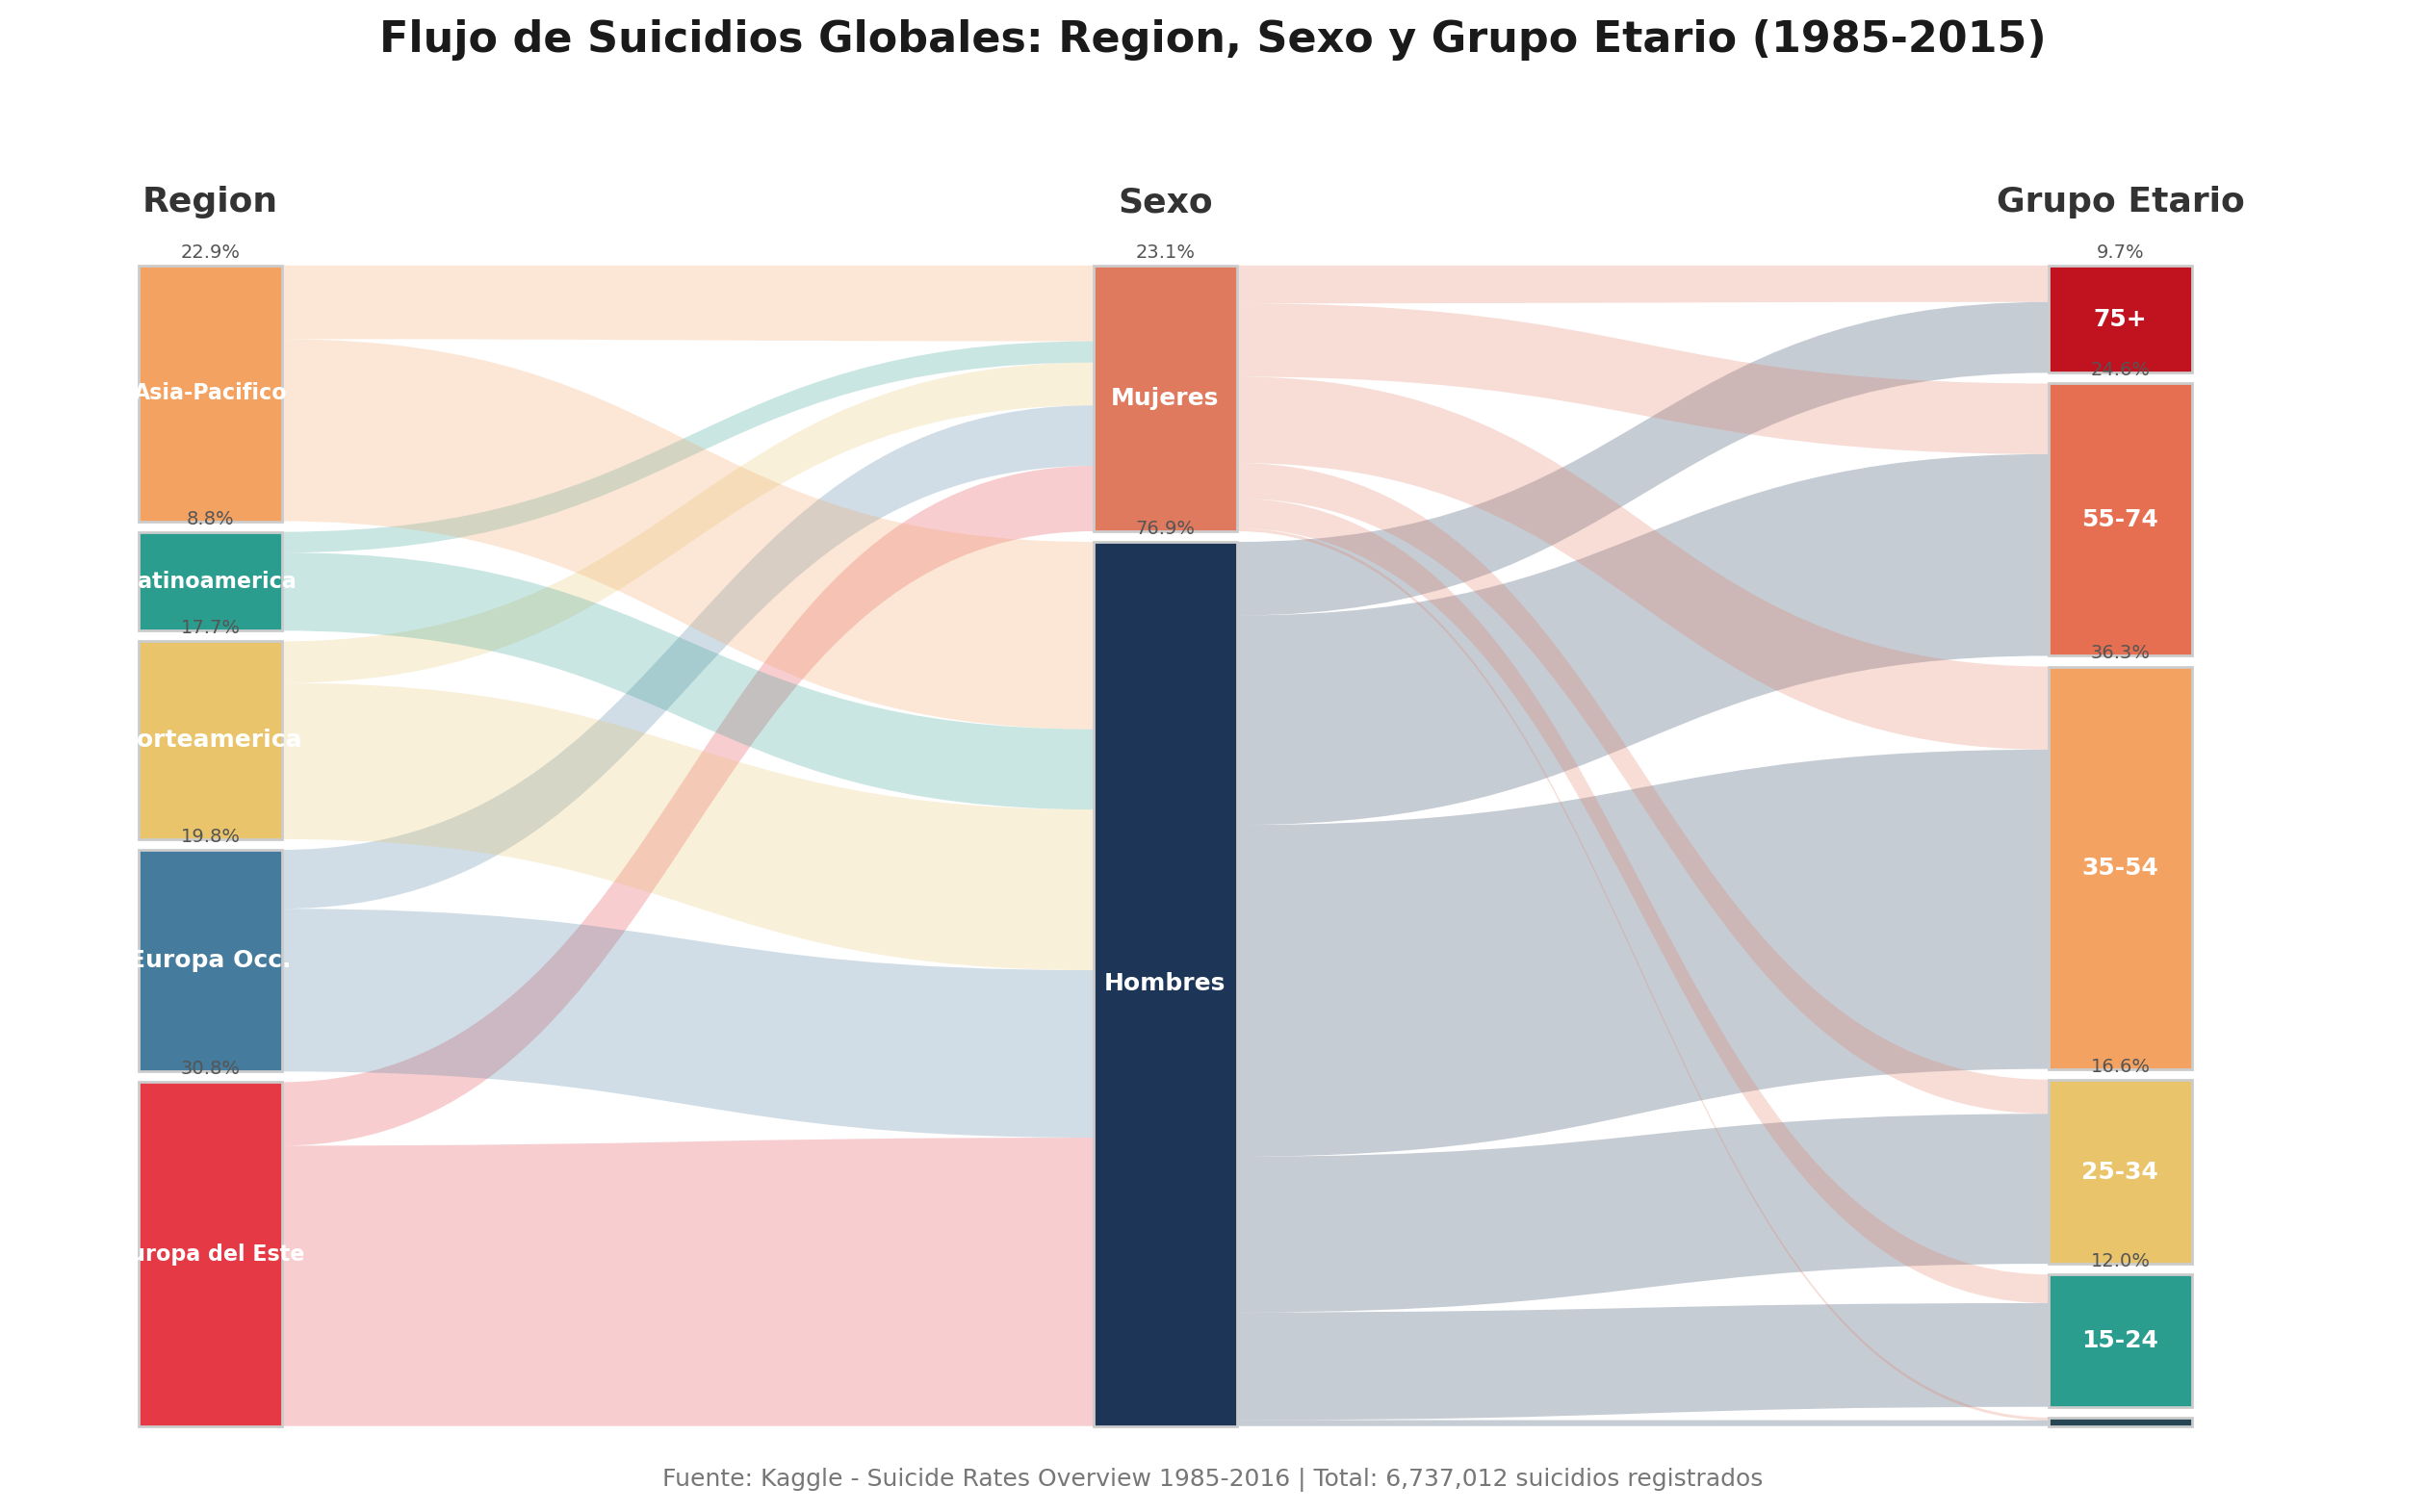
\includegraphics[width=0.95\textwidth]{figures/vis5_sankey.png}
  \caption{Diagrama de Sankey: Flujo de suicidios globales desde regi\'on hacia sexo y grupo etario (1985--2015). Fuente: Kaggle -- Suicide Rates Overview 1985--2016.}
  \label{fig:vis5_sankey}
\end{figure}

\subsubsection*{Ficha t\'ecnica}

\begin{table}[H]
  \centering
  \begin{tabularx}{\textwidth}{lX}
    \toprule
    \textbf{Elemento} & \textbf{Descripci\'on} \\
    \midrule
    Tipo de gr\'afico & Diagrama de Sankey (diagrama de flujo proporcional) \\
    Marca & \'Area (bloques proporcionales) + Enlace (curvas B\'ezier entre columnas) \\
    Canal -- Posici\'on X & Nivel categ\'orico: Regi\'on $\rightarrow$ Sexo $\rightarrow$ Grupo etario, variable categ\'orica jer\'arquica \\
    Canal -- Altura / Ancho del enlace & Volumen absoluto de suicidios, variable cuantitativa \\
    Canal -- Color (matiz) & Regi\'on de origen (5 categor\'ias) y sexo (2 categor\'ias), variables categ\'oricas nominales \\
    Esquem\'atica & Relacional: muestra c\'omo se distribuye el volumen total de suicidios a trav\'es de tres dimensiones categ\'oricas interconectadas \\
    Fuente de datos & Kaggle -- Suicide Rates Overview 1985--2016 \\
    \bottomrule
  \end{tabularx}
\end{table}

\subsubsection*{Conclusiones}

\begin{itemize}
  \item Europa del Este concentra la mayor proporci\'on de suicidios registrados (30,8\% del total global), superando ampliamente a regiones con mayor poblaci\'on como Asia-Pac\'ifico (22,9\%) o Norteam\'erica (10,0\%). Esto confirma a nivel de vol\'umenes absolutos lo que las tasas por 100k habitantes ya suger\'ian en las visualizaciones anteriores.
  \item La columna central revela que los hombres representan el 76,9\% de todos los suicidios registrados, y este dominio se mantiene consistente independientemente de la regi\'on de origen. La brecha de g\'enero es estructural y transversal a todas las regiones del mundo.
  \item El flujo hacia los grupos etarios muestra que las franjas de 35--54 y 55--74 a\~nos absorben conjuntamente m\'as del 55\% del total de suicidios, mientras que el grupo de 15--24 a\~nos (que la mayor\'ia de encuestados en la Tarea~2 identific\'o como el m\'as vulnerable) representa apenas el 13\%. Esto cierra el c\'irculo del hilo conductor del trabajo: la percepci\'on p\'ublica sobredimensiona el riesgo juvenil e invisibiliza a la poblaci\'on adulta y mayor.
\end{itemize}

% ─────────────────────────────────────────────────────────────────────────────

% ═════════════════════════════════════════════════════════════════════════════
\section{Resumen de responsabilidad individual}
% ═════════════════════════════════════════════════════════════════════════════

\begin{table}[H]
  \centering
  \caption{Detalle de responsabilidad por integrante.}
  \begin{tabularx}{\textwidth}{llXl}
    \toprule
    \textbf{Visualizaci\'on} & \textbf{Autor} & \textbf{Tipo de gr\'afico} & \textbf{Origen} \\
    \midrule
    Vis.\ 1 & Alexis Mellis    & Streamgraph            & Tarea 1 \\
    Vis.\ 2 & Andr\'es \'Aguila & Lollipop Divergente    & Tarea 2 \\
    Vis.\ 3 & Alexis Mellis    & Mapa Coropleta         & Tarea 3 \\
    Vis.\ 4 & Alexis Mellis    & Bump Chart             & Nueva \\
    Vis.\ 5 & Andr\'es \'Aguila & Diagrama de Sankey    & Nueva \\
    \bottomrule
  \end{tabularx}
\end{table}

% ═════════════════════════════════════════════════════════════════════════════
\section{Conclusiones generales}
% ═════════════════════════════════════════════════════════════════════════════

Este trabajo pr\'actico cierra el an\'alisis del macrotema \textbf{Muerte} integrando las dimensiones exploradas a lo largo de las tres tareas previas con dos nuevas visualizaciones que profundizan en la din\'amica del fen\'omeno.

El Streamgraph (Tarea~1) estableci\'o la base temporal mostrando c\'omo la distribuci\'on etaria de los suicidios evoluciona a lo largo de tres d\'ecadas, con un ensanchamiento transversal alrededor del a\~no 2000. El Lollipop Divergente (Tarea~2) a\~nadi\'o la dimensi\'on perceptual, revelando que la percepci\'on p\'ublica sobre la proporci\'on femenina en suicidios duplica la realidad estad\'istica. El Mapa Coropleta (Tarea~3) anclaba estas cifras en el territorio, confirmando la concentraci\'on en Europa del Este y Asia Central.

Las dos visualizaciones nuevas completan este panorama desde \'angulos complementarios. El Bump Chart rastrea la competencia entre pa\'ises por las posiciones m\'as altas del ranking, demostrando que el bloque post-sovi\'etico no solo lidera en tasas absolutas sino que mantiene esa hegemon\'ia de forma sostenida durante 30 a\~nos. El Diagrama de Sankey descompone los casi 7 millones de suicidios registrados en tres ejes simult\'aneos (regi\'on, sexo, grupo etario), haciendo visible de forma inmediata que el perfil t\'ipico del suicidio a nivel global es masculino, adulto y concentrado en regiones de transici\'on socioecon\'omica.

En conjunto, las cinco visualizaciones convergen en una conclusi\'on central: el suicidio no es un fen\'omeno aleatorio ni uniforme, sino un problema estructural con patrones geogr\'aficos, demogr\'aficos y de g\'enero claramente identificables, cuya comprensi\'on p\'ublica dista significativamente de la realidad que revelan los datos.

% ═════════════════════════════════════════════════════════════════════════════
\section{Repositorio de GitHub}
% ═════════════════════════════════════════════════════════════════════════════

El c\'odigo fuente de todas las visualizaciones se encuentra disponible en el siguiente repositorio:

\begin{center}
  \href{https://github.com/siroale/VisualizacionDeDatos-2026-01}{\texttt{https://github.com/siroale/VisualizacionDeDatos-2026-01}}
\end{center}

\begin{verbatim}
/
|-- Code/
|   |-- Alexis-Mellis/
|   `-- Andres-Aguila/
|-- Datasets/
|   |-- suicide_dataset.csv
|   `-- encuesta.csv
|-- Informe_1/
|-- Informe_2/
|-- Informe_3/
|-- Informe_TP/
|   |-- figures/
|   |-- informe.pdf
|   `-- informe.tex
`-- README.md
\end{verbatim}

\end{document}
